% Figure from MATH 556 notes, section 33. Compile with the notes preamble.
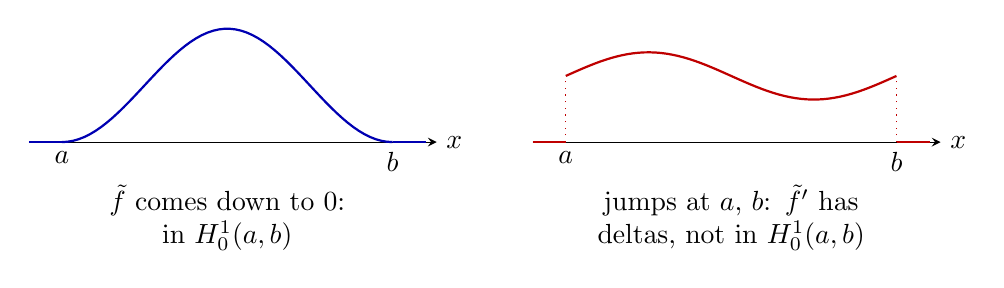
\begin{tikzpicture}[x=1.4cm, y=1.2cm, >=stealth]
    \begin{scope}
        \draw[->] (-0.3,0) -- (3.4,0) node[right] {$x$};
        \draw[thick, blue!70!black, domain=0:3, samples=60] plot (\x, {1.2*sin(60*\x)^2});
        \draw[thick, blue!70!black] (-0.3,0) -- (0,0); \draw[thick, blue!70!black] (3,0) -- (3.3,0);
        \node[below] at (0,0) {$a$}; \node[below] at (3,0) {$b$};
        \node[below, text width=4cm, align=center] at (1.5,-0.35) {$\tilde f$ comes down to $0$: \\ in $H^1_0(a,b)$};
    \end{scope}
    \begin{scope}[xshift=6.4cm]
        \draw[->] (-0.3,0) -- (3.4,0) node[right] {$x$};
        \draw[thick, red!75!black, domain=0:3, samples=60] plot (\x, {0.7+0.25*sin(120*\x)});
        \draw[thick, red!75!black] (-0.3,0) -- (0,0); \draw[thick, red!75!black] (3,0) -- (3.3,0);
        \draw[dotted, red!75!black] (0,0) -- (0,0.7); \draw[dotted, red!75!black] (3,0) -- ({3},{0.7+0.25*sin(360)});
        \node[below] at (0,0) {$a$}; \node[below] at (3,0) {$b$};
        \node[below, text width=4cm, align=center] at (1.5,-0.35) {jumps at $a$, $b$: $\tilde f'$ has \\ deltas, not in $H^1_0(a,b)$};
    \end{scope}
\end{tikzpicture}
